\documentclass[14pt,russian]{extreport}
\usepackage[utf8]{inputenc}
\usepackage{geometry}
%\geometry{verbose,tmargin=2cm,bmargin=2cm,lmargin=2cm,rmargin=2cm}
\geometry{verbose,tmargin=2.0cm,bmargin=2.0cm,lmargin=3.0cm,rmargin=2.0cm}
%\geometry{verbose,tmargin=3cm,bmargin=3cm,lmargin=3cm,rmargin=3cm}

\usepackage{amssymb}
\usepackage{setspace}
\usepackage{babel}
\usepackage{color}
\usepackage[hidelinks]{hyperref}
\usepackage{natbib}
%\usepackage{authordate1-4}
%\bibliographystyle{authordate1}
\bibliographystyle{unsrt}
\usepackage{amsmath}
\newtheorem{hyp}{Гипотеза}
\usepackage[draft]{graphicx}
\graphicspath{img/}
\usepackage{float}
\usepackage{placeins}
\usepackage{chngcntr}
\counterwithout{figure}{chapter}
\counterwithout{table}{chapter}
\usepackage{multicol}

\usepackage{CJKutf8}
%\onehalfspacing
\linespread{1.5}

% remove chapter number from section headings
\renewcommand*\thesection{\arabic{section}}

\usepackage{amsmath}
\DeclareMathOperator*{\argmin}{argmin}
\DeclareMathOperator*{\argmax}{argmax}
\newcommand*{\argminl}{\argmin\limits}
\newcommand*{\argmaxl}{\argmax\limits}

% rename chapters
\makeatletter
\renewcommand{\@chapapp}{Глава}
\makeatother

% continuous equation numbering through chapters
\usepackage{chngcntr}
\counterwithout{equation}{chapter}

\usepackage{amsthm}
\theoremstyle{definition}
\newtheorem{definition}{Определение}[subsection]

\usepackage{indentfirst}
\frenchspacing

\newcommand{\todo}[1]{}
\renewcommand{\todo}[1]{{\color{red} TODO: {#1}}}

\begin{document}
	
\begin{titlepage}
	\begingroup
	\centering
	{\scshape
		\fontsize{12pt}{14pt}\selectfont Министерство образования и науки Российской Федерации\par
		\vspace{0.7cm}
		Государственное образовательное учреждение \\высшего профессионального образования\par
		Московский физико-технический институт\\(государственный университет)\par
		\vspace{0.7cm}
		Факультет инноваций и высоких технологий\par
		Кафедра компьютерной лингвистики\par
		\vspace{0.7cm}
		\fontsize{14pt}{17pt}\selectfont выпускная квалификационная работа\\(бакалаврская работа)\par}
	\fontsize{14pt}{17pt}\selectfont по направлению 01.03.02 «Прикладная математика и информатика»\par
	\vspace{1cm}
	{\fontsize{21pt}{25pt}\selectfont\bfseries Японский. Буквенные n-грамы \\ для распознавания\par}
	\vspace{4cm}
	
	\begin{tabular}{l@{\hspace{140pt}}r}
		Студент & Куликов А.В. \\
		Научный руководитель & Андрианов А.И.
	\end{tabular}
	\par
	\vfill
	
	{\fontsize{14pt}{17pt}\selectfont Москва, 2017\par}
	\endgroup
\end{titlepage}
\onehalfspacing

\addtocounter{page}{1}
\tableofcontents{}

\newpage
\section*{Введение}
\addcontentsline{toc}{section}{Введение}

История попыток распознать текст началась более века назад. В 1914 году Эмануэль Гольдберг разработал устройство, которой считывало символы и транслировало их в телеграфный код. Примерно в то же время ирландский химик Эдмунд Фурнье д’Альбе создал и запатентовал «оптофон» — прибор, умеющий переводить написанное в систему звуков, различающихся по высоте. Оптофон предназначался для того, чтобы слепые могли «читать».

В 1929 году Густав Таушек (Gustav Tauschek) разработал метод оптического распознавания текста. Машина Таушека представляла собой механическое устройство, которое использовало шрифтовые шаблоны и фотодетектор. Он запатентовал своё изобретение сначала в Германии, а позднее и в США, в 1935 году. Это и положило начало проблеме качественного оптического распознавания символов (Optical Character Recognition, OCR).

Коммерческое производство подобных маних было налажено уже в 1950-х, после войны. Использовавшие наработки военных, производители OCR-машин продвигались всё дальше, увеличивая применимость технологии и качество распознавания.

Постепенно появлялись как универсальные OCR-программы (ABBYY FineReader, Adobe Acrobat), так и специализированные для конкретной области (SmartScore для нотной записи, Persian Reader для фарси и т.д.). При этом точность в задаче распознавания напечатанных латинских символов достигла 99\%-100\% качества, в то время как корректное распознавание рукописного текста или текста, написанного в другом алфавите, до сих пор является темой множества исследований. Особняком стоит задача распознавания текста на восточных языках (китайский, японский, корейский, ...), из-за большого размера алфавита в этих языках.

Настоящая работа представляет собой сравнение некоторых методов машинного обучения для исправления ошибок распознавания текста в японском языке. 

Спектр способов, которыми можно решать проблему автоматического исправления ошибок, довольно широк, и включает в себя различные вариации $n$-граммных методов ($n$-gram models), использование нейросетей (Neural Networks, NN), скрытых моделей Маркова (Hidden Markov Models, HMM) и прочих методов машинного обучения. Более подробный обзор основных современных подходов можно найти в \cite{das:survey}.
 
Среди возможных решений использование $n$-граммных моделей занимает особую нишу из-за относительной прозрачности и интуитивности принципов работы, и в то же время достаточно широких возможностей по настройке алгоритма.

Подход, предложенный в \cite{nagata:shape}, использует $n$-граммные модели, а также различные алгоритмы сглаживания для исправления опечаток, опираясь на словное деление текста. 

В работе \cite{nagata:context} также даются эвристики для определения границ слов, использующие граф линейного деления (ГЛД). Эти границы слов затем используются в $n$-граммной модели в качестве вспомогательного контекста.

Более подробно эти и другие подходы разобраны в соответствующем разделе (\ref{sec:litreview}).

Данное исследование призвано рассмотреть некоторые из $n$-граммных моделей и сравнить их эффективность в задаче исправления опечаток в японском языке.

Актуальным приложением этой работы является система распознавания восточных языков в ABBYY FineReader.

\newpage

\section{ Постановка задачи }\label{sec:taskdef}

\begin{definition}{\textit{Оптическое распознавание символов (Optical Character Recognition, OCR)}} -- процесс считывания текста с физического носителя и его сохранения в цифровом формате. Текст состоит из \textit{символов}.
\end{definition}

\begin{definition}{\textit{Ошибка OCR}} -- случай, когда очередной символ текста распознался неверно или не распознался. Ведёт к понижению качества распознавания.
\end{definition}

\begin{definition}{\textit{$N$-грамма}} -- последовательность из $n$ элементов (слов, звуков, символов). Анализируя их частотности, можно строить модели для анализа и синтеза языка.
\end{definition}

\begin{definition}{\textit{$N$-граммная модель}} -- вероятностная модель языка, которая рассчитывает вероятность последнего элемента $n$-граммы, если известны все предыдущие. \\
При использовании $n$-граммных моделей предполагается, что появление каждого элемента зависит только от предыдущих элементов.
\end{definition}

\textbf{Цель работы} -- сравнить эффективность различных символьных $n$-граммных моделей в задаче исправления ошибок OCR в японском языке.

Из цели работы вытекают следующие \textbf{задачи}:
\begin{itemize}
	\item Рассмотреть существующие подходы к $n$-граммному моделированию японского языка;
	
	\item Реализовать некоторые символьные $n$-граммные модели;
	
	\item Развернуть систему для тестирования и сравнения моделей.
\end{itemize}

Чтобы понять специфику цели работы, нужно учесть особенности японского языка.

Очевидно, что устройство японского языка на уровне конкретных символов сложнее, чем устройство языков латино-романской группы, в которых существует всего 25-40 символов, учитывая возможную диакритику.

\subsection{ Обзор японского языка }
\label{sec:japanese}

Письменный японский текст -- это комбинация слогово-фонетических символов (кана) и иероглифов (кандзи).
Слоговая азбука кана делится на катакану и хирагану, которые представляют собой разные графические формы одних и тех же слогов.

Рассмотрим эти символы подробнее:

\begin{itemize}
	\item Хирагана (см. \cref{fig:hirag_sample}). В основном используется для образования грамматических морфем.
	\begin{figure}[H]
		\centering
		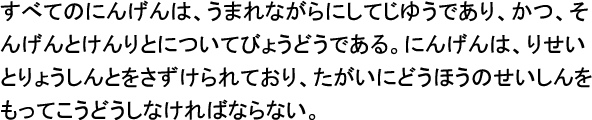
\includegraphics{hirag_sample.png}
		\caption{Хирагана}
		\label{fig:hirag_sample}
	\end{figure}
	
	\item Катакана (см. \cref{fig:katak_sample}). Используется для транскрибирования иностранных заимствованных слов.
	\begin{figure}[H]
		\centering
		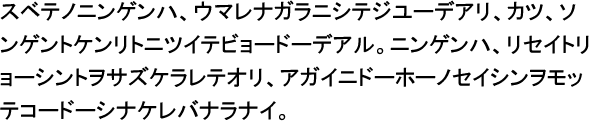
\includegraphics{katak_sample.png}
		\caption{Катакана}
		\label{fig:katak_sample}
	\end{figure}

\newpage
	\item Также есть диакритические символы -- дакутен, хандакутен (см. \cref{fig:dakut_sample_hir} и \cref{fig:dakut_sample_kat}). Они могут применяться как к катакане, так и к хирагане, и определённым образом влияют на звучание слогов.
	\begin{multicols}{2}
		
		\begin{figure}[H]
			\centering
			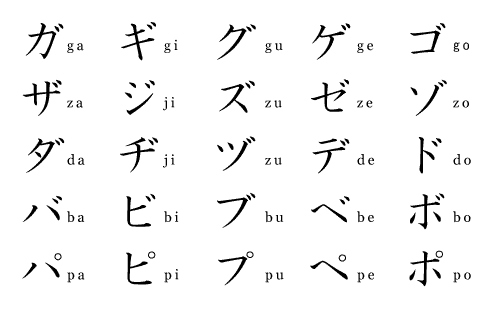
\includegraphics[scale=0.6]{dakut_sample.png}
			\caption{Дакутен катакана}
			\label{fig:dakut_sample_hir}
		\end{figure}
		
		\begin{figure}[H]
			\centering
			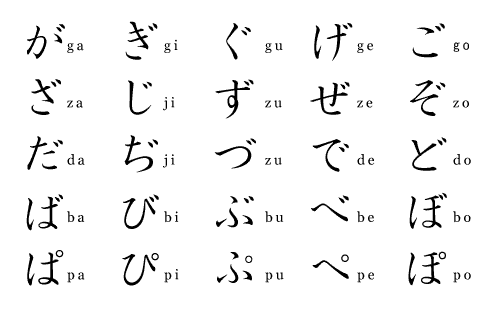
\includegraphics[scale=0.6]{handakut_sample.png}
			\caption{Дакутен хирагана}
			\label{fig:dakut_sample_kat}
		\end{figure}
		
	\end{multicols}
	
	\item Кандзи (см. \cref{fig:kandji_sample}). Это символы, несущие семантическую нагрузку.
	\begin{figure}[H]
		\centering
		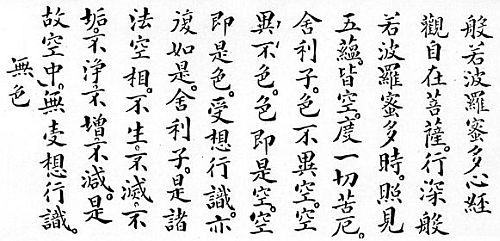
\includegraphics{kanji_sample.png}
		\caption{Кандзи}
		\label{fig:kandji_sample}
	\end{figure}
\end{itemize}

Кана различает 46 слогов, которые могут записываться как катаканой, так и хираганой. А вот иероглифов кандзи существует гораздо больше: 2136 (т.н. jōyō kanji -- "обычно используемые кандзи") достаточно для жизни, 6879 используется в кодировке JIS X 0208 (Japanese Industrial Standart, см. \cite{JISX0208}), а самые большие словари иероглифов (например, Большой китайско-японский словарь) включают в себя от 50000 до 85000.

Кроме перечисленных символов, в японском тексте могут быть и другие: фуригана -- маленькие знаки каны в качество фонетических подсказок, ромадзи -- система транслитерации японских слов в латиницу и т.д. Однако, в данной работе эти разделы оставлены за кадром.

Японский текст записывается с помощью комбинаций кандзи, кан и пунктуации, при этом отсутствует пробельное деление предложений на слова (см. \cref{fig:japtext_sample}).
	\begin{figure}[H]
	\centering
	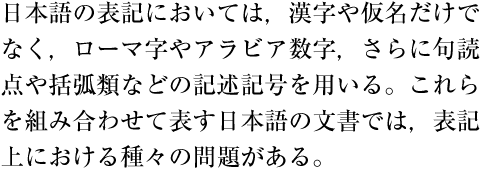
\includegraphics{japtext_sample.png}
	\caption{Японский текст}
	\label{fig:japtext_sample}
\end{figure}

По сравнению с латино-романскими языками, где алфавит меньше в сотни раз, а деление текста на слова очевидно, задача корректного распознавания символов становится значительно сложнее. Это требует более изощрённых подходов для автоматического анализа распознанного текста и поиска ошибок в нём.

Рассмотрим несколько примеров символов, которые легко спутать.

\subsection{ Путающиеся символы в японском }

При таком большом размере алфавита частые ошибки OCR можно разбить по классам. Вот некоторые из них:

\begin{itemize}
	\item[\textbf{2Kana}] 2 похожие каны. Таких случаев достаточно мало, а методы их различения уже существуют (см., например, метод с использованием глубокого обучения и свёрточных нейронных сетей в работе \cite{tsai:dcnn}).
	\begin{figure}[H]
		\center{\raisebox{-.5\height}{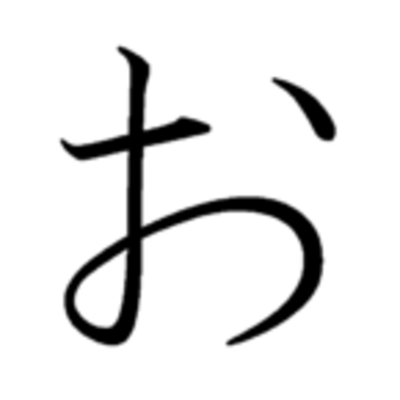
\includegraphics[height=100pt]{KanaO.png}}\ и \raisebox{-.5\height}{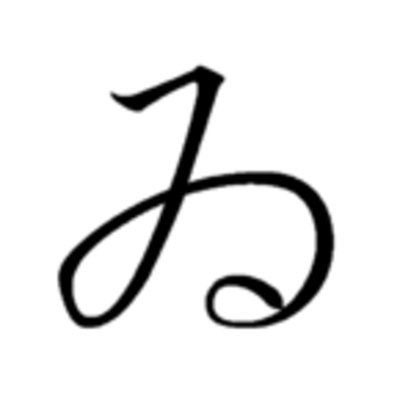
\includegraphics[height=100pt]{KanaWi.png}}}
	\end{figure}

	\item[\KG] Кана может легко путаться с соответствующим ей дакутен-символом.
	\begin{figure}[H]
		\center{\raisebox{-.5\height}{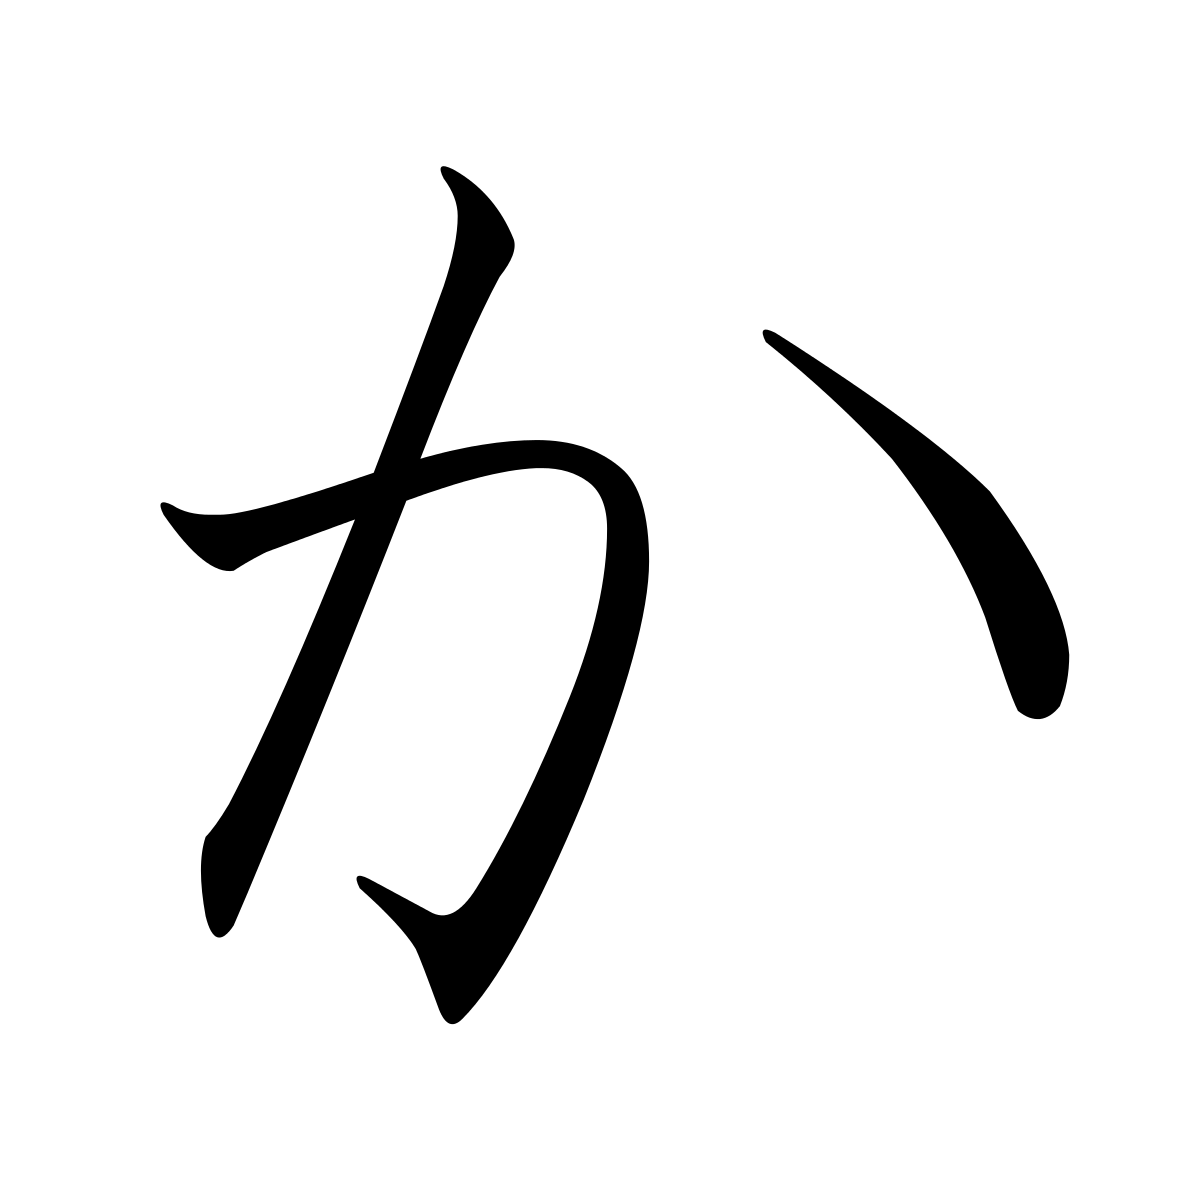
\includegraphics[height=100pt]{KanaKa.png}}\ и \raisebox{-.5\height}{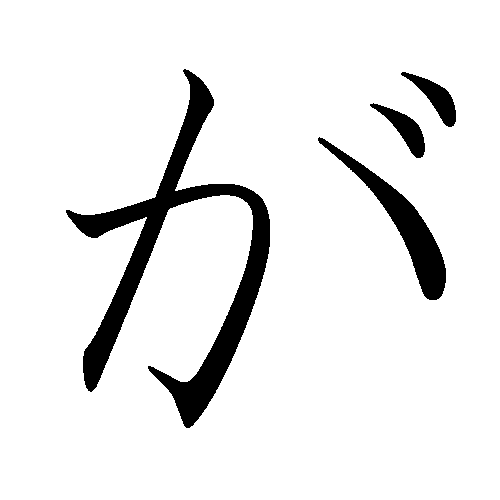
\includegraphics[height=100pt]{KanaGa.png}}}
	\end{figure}

	\item[\BS] Существуют большие и маленькие каны, которые нужно различать.
	\begin{figure}[H]
		\center{\raisebox{-.5\height}{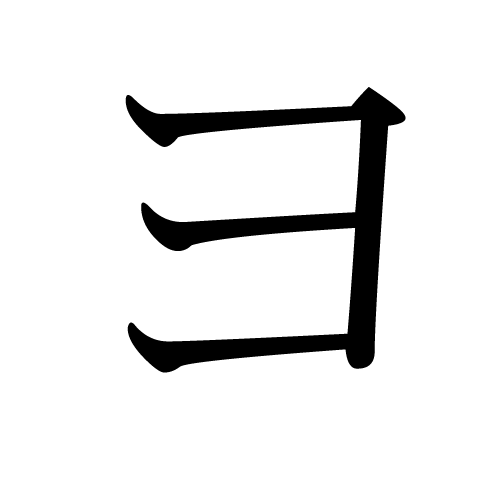
\includegraphics[height=100pt]{KanaYo.png}}\ и \raisebox{-.5\height}{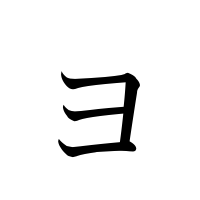
\includegraphics[height=100pt]{KanaYoSmall.png}}}
	\end{figure}
	
\end{itemize}

В будущем мы будем рассматривать 3 случая ошибок: \textbf{\KG}, \textbf{\BS} и \textbf{\MX} (смесь \textbf{\KG} и  \textbf{\BS} ), более строгое определение которых будет дано в \cref{sec:experiment}.

\subsection{ Формальная постановка задачи }

\begin{definition}
	{\textit{Алфавит $\Sigma = \{ a, b, c, .. \}$}} -- множество символов в данном языке.
\end{definition}

\begin{definition}
	{\textit{Текст $Text \in \Sigma^+$}} -- последовательность символов из алфавита $\Sigma$ положительной длины.
\end{definition}

\begin{definition}
	Текст делится на конечное число {\textit{предложений $S = \{ S_1, S_2, S_3, ... \}$}} знаками пунктуации и форматированием. $Text = S_1S_2S_3...$.
\end{definition}

Для каждого из предложения текста существует единственно верный вариант написания, а также некоторое (фиксированное) число неверных. Требуется ответить, какой из вариантов верен.

\begin{definition}
	{\textit{Оценивающий алгоритм (estimator) $\Theta : S \rightarrow \mathbb{R}^+ $}} -- функция, возвращающая оценку правильности варианта $S$.
\end{definition}

Среди $k$ вариантов предложения выбирается наилучший: $S_{best} = \argmaxl_{S} \Theta(S)$, который и считается правильным.

Если $S_{best}$ угадано верно, то на данном предложении алгоритм $\Theta$ отработал правильно.

\begin{definition}
	{\textit{Качество алгоритма $Q(\Theta) = \dfrac{\#\{ \text{угаданных предложений} \}}{\#\{ \text{всего предложений} \}}$}}.
\end{definition}

Задача -- реализовать ряд оценивающих алгоритмов (см. \cref{sec:models}), основанных на $n$-граммных моделях, и сравнить их по качеству.

\newpage
\section{ Обзор источников }\label{sec:litreview}

Проблема качественного OCR в различных языках (в частности, в японском) стоит достаточно давно, и существует множество различных подходов к её решению. Большинство подходов основываются на применении различных методов машинного обучения, такие как $n$-граммные модели, нейросети, модели Маркова и т.д. 

В силу особенностей японского языка (см. \cref{sec:japanese}), а именно отсутствия словного деления в текстах, существующие методы исправления ошибок OCR можно разделить на 2 класса: использующие информацию о словном делении и не использующие её.

\subsection{ Методы, не использующие словное деление }

Идея подобных методов заключается в том, чтобы, не тратя ресурсы на определение границ слов в тексте, оперировать предложениями (границы которых выделяются достаточно легко) как единицами трансляции, и исправлять возможные ошибки OCR, не углубляясь в членение предложений.

\todo{примеры статей?}

Стоит также заметить, что настоящая работа может быть отнесена к этому классу.

\subsection{ Методы, использующие словное деление }

Информация о словном делении текста даёт удобный контекст для выделения признаков и настройки параметров при машинном обучении. Но эту информацию надо откуда-то получать, что приводит к делению алгоритмов на 2 этапа:

\begin{itemize}
	\item Получение словного деления. Может производиться с помощью специализированных алгоритмов (например, модификаций алгоритма Витерби, как в \cite{nagata:context}, или марковских случайных полей (conditional random fields, CRFs), как в \cite{kudo:crfs}), а также путём анализа конкретных языковых конструкций (например, bunsetsu boundaries, см. \cite{chung:bunsetsu}).
	
	Кроме того, словное деление может быть получено путём использования в работе предварительно размеченного корпуса, в разметке которого есть словное деление. В качестве примеров таких корпусов можно привести EDR Japanese Corpus (см. \cite{corpus:edr}), ATR Dialogue Database (см. \cite{corpus:atr}) и т.д.
	
	\item Применение словного деления как контекста для детектирования ошибок OCR. Достоверная информация о словном делении позволяет считать слова единицами трансляции, не теряя контекста предложения. Это даёт возможность получить больше признаков для машинного обучения. Подобный подход представлен в статье \cite{nagata:shape}, где используются $n$-граммные модели с backoff и различными подходами к сглаживанию (Good-Turing, Witten-Bell). 
\end{itemize}

Обзору основных актуальных методов исправления ошибок OCR в японском также целиком посвящена статья \cite{das:survey}.

\newpage
\section{ Описание моделей оценивания текста }\label{sec:models}

Перед обучением моделей корпус разбивается на независимые и гомогенные части: обучающую и тестовую выборки. Обучающая выборка используется для обучения модели, тестовая -- для проверки качества обучения и, собственно, оценки модели.

В работе рассматриваются следующие модели: 

\begin{itemize}
	\item $n$-граммные с фиксированным $n,\ n \in \{1,2,3\}$
	
	\item Backoff-модель, $n_{max} \in \{ 3, 5, 7 \}$
	
	\item Модель Катца (Katz),  $n_{max} \in \{ 3, 5, 7 \}$
\end{itemize}

Также из-за большого размера алфавита необходимо использовать сглаживание (smoothing) для учёта символов и $n$-грамм, не встретившихся в обучающей выборке. Подробнее о механизме сглаживания -- см. раздел \cref{sec:experiment}.

Во всех моделях оценка предложения производится через агрегацию оценок отдельных $n$-грамм.

\subsection{ $N$-граммные модели с фиксированным $n$ }

\paragraph{ Обучение модели } Для данного $n$ по обучающей выборке собираются статистики по всем $n$-граммам. Эти статистики затем нормализуются и сериализуются для дальнейшего использования.

$$ C(x_{i - n + 1}, ..., x_{i - 1}, x_i) = \dfrac{N(x_{i - n + 1}, ..., x_{i - 1}, x_i)}{N(x_{i - n + 1}, ..., x_{i - 1})} $$ 

\paragraph{ Применение модели } В силу простоты модели оценка $n$-граммы из тестовой выборки берётся напрямую из собранных на предыдущем этапе статистик.

$$ P(x_i | x_{i - n + 1}, ..., x_{i - 1}) = C(x_{i - n + 1}, ..., x_{i - 1}, x_i) $$

\subsection{ Backoff-модель } 

\paragraph{ Обучение модели } Этап обучения модели практически такой же, как и в случае простой $n$-граммной модели, с разницей в том, что здесь собираются статистики для всех $n \leq n_{max}$.

\paragraph{ Применение модели } Идея backoff-подхода состоит в том, что при нехватке данных для оценки какой-либо $n$-граммы $x_{i - (n - 1)} ... x_{i - 1} x_i$ постепенно уменьшается $n$, что позволяет увеличить общность алгоритма и оценить $n$-грамму по частям, но более надёжно. За счёт этого уменьшается вероятность переобучения модели на конкретных данных. Подробнее можно узнать в \cite{manning}.

\[ P_n(x_i | x_{i - n + 1}, ..., x_{i - 1}) =
\begin{cases}
	C(x_i | x_{i - n + 1}, ..., x_{i - 1})       & \quad \text{if } C(x_i | x_{i - n + 1}, ..., x_{i - 1}) > k\\
	P_{n - 1}(x_i | x_{i - n + 2}, ..., x_{i - 1})  & \quad \text{otherwise }\\
\end{cases}
\]

\subsection{ Модель Катца (Katz) }

\paragraph{ Обучение модели } Этап обучения модели такой же, как и в случае backoff-модели.

\paragraph{ Применение модели } Модель Катца является улучшенной версией backoff-модели, в которой накладывается динамический дисконт (коэффициенты $d_{w_{i-n+1}...w_i}$ и $\alpha_{w_{i-n+1}...w_{i-1}}$) на оценку $n$-граммы в случае уменьшения $n$. Более подробно о модели Катца можно прочитать в \cite{katz:backoff}.

\[
P_{n}\left( w_i | w_{i-n+1}...w_{i-1} \right) = 
\begin{cases}
d_{w_{i-n+1}...w_i} \dfrac{C(w_{i-n+1}...w_i)}{C(w_{i-n+1}...w_{i-1})} &\text{if $C(w_{i-n+1}...w_i) > k$}\\
\alpha_{w_{i-n+1}...w_{i-1}} P_{n - 1}\left( w_i | w_{i-n+2}...w_{i-1} \right) &\text{otherwise}
\end{cases}
\]

При этом коэффициенты $d_{w_{i-n+1}...w_i}$ и $\alpha_{w_{i-n+1}...w_{i-1}}$ вычисляются следующим образом:

$$d_{w_{i-n+1}...w_i} - \text{ размер дисконта, вызванного сглаживанием (см. \cref{sec:experiment}) }$$

$$\alpha_{w_{i-n+1}...w_{i-1}} - \text{ размер дисконта за backoff } -$$ 
$$ = \dfrac{\beta_{w_{i-n+1}...w_{i-1}}}{\Sigma_{\{ w_i : C(w_{i-n+1}...w_{i-1}) \leq k \}} P_{n-1}\left( w_i | w_{i-n+2}...w_{i-1} \right)}\text{,}$$

$$\text{где } \beta_{w_{i-n+1}...w_{i-1}} - \text{ остаточная плотность вероятности для ($n-1$)-грамм } - $$
$$ = 1 - \Sigma_{\{ w_i : C(w_{i-n+1}...w_{i}) > k \}} \dfrac{C(w_{i-n+1}...w_i)}{C(w_{i-n+1}...w_{i-1})} $$ \todo{проверить N или C тут}


\newpage
\section{ Описание эксперимента }\label{sec:experiment}

Для исследования способов исправлять ошибки OCR в тексте необходимо либо иметь большой корпус размеченных данных с результатами распознавания, либо как-то выкручиваться. 

Пришлось выкручиваться, эмулируя ошибки OCR самостоятельно.

\todo{Описание машины -- в приложение}

\subsection{ Корпус }

Для обучения и сравнения $n$-граммных моделей использовался корпус html-страниц с ряда японских сайтов (\todo{Каких? Где?}) общим размером $\approx 8,5 GB$. 

Тексты из этого корпуса не были результатом OCR, поэтому в них не должно было быть ошибок, связанных с распознаванием. Эти тексты были признаны верными с точки зрения языка и подходящими для обучения моделей.

В рамках подготовки корпуса к эксперименту тексты были перемешаны, чтобы тематика текста не зависела от его исходного положения в корпусе, из текстов были удалены html-теги, сложное форматирование, небольшое число мусорных символов. Также корпус был единообразно переведён в кодировку Unicode. Подробнее об этих технических этапах -- см. раздел \ref{sec:coding}.

После вышеперечисленных операций корпус был готов к использованию, его размер составлял $\approx 1,5 GB$. При этом размер алфавита в нашем корпусе составлял $\approx 7000$ символов, что в 3 раза меньше размера таблиц Unicode.

Имея данные, готовые к использованию, было бы глупо не построить по ним несколько графиков.

\subsection{ \todo{Zipf} }

Если посмотреть на распределение частот отдельных символов, то оно выглядело так:

\begin{figure}[H]
	\centering
	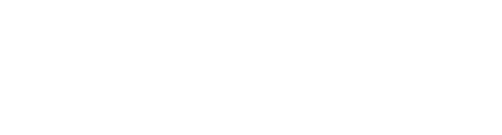
\includegraphics{draft.png}
	\caption{1gramstats}
	\label{fig:1gramstats_all}
\end{figure}

Видно, что распределение похоже на обратно экспоненциальное (кстати, это же утверждает закон Ципфа \todo{link}). Проверим эту гипотезу, построив график обратного логарифма (\todo{формулы}):

\begin{figure}[H]
	\centering
	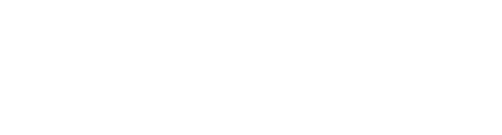
\includegraphics{draft.png}
	\caption{zipf}
	\label{fig:zipf1gram}
\end{figure}

Действительно, этот график с достаточной точностью ложится на прямую (\todo{погрешности?}). Тем самым, в NLP закон Ципфа проверен ещё раз.

Посмотрев на Рис. \ref{fig:1gramstats_all}, можно также заметить, что только очень малая часть символов появляется большое число раз. Посмотрим поближе на "голову"\ того же распределения:

\begin{figure}[H]
	\centering
	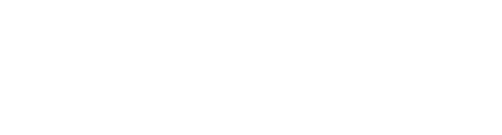
\includegraphics{draft.png}
	\caption{1gramstats head}
	\label{fig:gramstats_head}
\end{figure}

Действительно, лишь $\approx 200$ символов встречаются достаточно часто.

Осталюся ещё примерно $6500$ символов, которые входят в алфавит, но статистически мало отличаются от тех символов, что вовсе не встретились в нашем корпусе. Для оптимизации времени работы и занимаемой памяти эти символы можно представить более сжато.

\begin{definition}
	{\textit{Корзина (бакет, bucket)}} -- множество символов, которые считаются статистически малозначимыми и заменяются на U+FFFD (Unicode Replacement Character).
\end{definition}

Бакет $B_i$ характеризуется числом $|\Sigma_{B_i}|$ -- размером алфавита, который остаётся после сливания некоторого хвоста распределения в бакет. Было решено рассматривать бакеты с алфавитами размером $|\Sigma_{B_i}| = \{ 7000, 4800, 2600, 200 \}$, поскольку примерно на эти размеры алфавитов приходятся изменения в характере убывания частот символов.

На Рис. \ref{fig:bucket_pic} схематично изображено распределение частот после применения бакета с $|\Sigma_{B_i}| = 200$.

\begin{figure}[H]
	\centering
	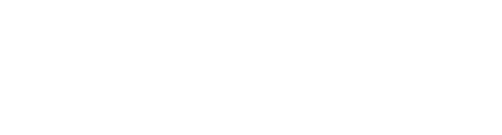
\includegraphics{draft.png}
	\caption{bucket}
	\label{fig:bucket_pic}
\end{figure}

Поскольку нам были недоступны корпуса текстов, распознанные какой-либо OCR машиной, было принято решение эмулировать ошибки OCR самим. Это делалось при помощи генератора шума.

\subsection{ Генератор шума и режимы его работы }

\begin{definition}
	{\textit{Шум $Noise = \{ (a_1, a_2), (b_1, b_2, b_3), (c_1, c_2), ... \}$}} -- множество наборов символов алфавита $\Sigma$, которые легко спутать при распознавании. Конкретные шумы определяются эмпирически. 
\end{definition}

Для эмуляции ошибок OCR был разработан скрипт -- генератор шума. Он параметризуется конкретным шумом и частотой его применения.

\begin{definition}
	{\textit{Генератор шума}} -- настраиваемый скрипт, который принимает эталонное предложение $S$, находит в нём символы-представители наборов конкретного шума $x \in S\ |\ \exists \xi = \{ \xi_1, \xi_2, ..., \xi_l \} \in Noise : x \in \xi$, и случайным образом меняет эти символы $x$ на "шумовые" из соответствующего набора $\xi$.
\end{definition}

С помощью шума $Noise$ случайным образом генерируются ошибки в предложениях текста $Text$. Таким образом происходит стохастическая эмуляция ошибок OCR. 

Тестовая часть корпуса была разбита на предложения (см. формальную постановку задачи в разделе \ref{sec:taskdef}), которые независимо друг от друга зашумлялись. Эти предложения после зашумления подавались на вход оценивающему алгоритму $\Theta$, который выбирал лучший из предложенных вариантов.

Были определены следующие шумы, обоснование выбора см. в разделе \ref{sec:taskdef}: 

\begin{itemize}
	\item[KaGa] Наборы симвопов, соответствующие добавлению диакритики. Например,
	
	\begin{multicols}{3}
		\begin{CJK}{UTF8}{min}
			かが \\
			きぎ \\
			くぐ \\
			けげ \\
			こご \\
			さざ \\
			しじ \\
			すず \\
			ふぶぷ   \\
			そぞ \\
			ただ \\
			なに \\
			たな \\
			だな \\
			んだ \\
			ちぢ \\
			つづ \\
		ほぼぽ \end{CJK}
	\end{multicols}
	
	\item[HalfWidth] Полуширинные/полноширинная катакана:
	
		\begin{multicols}{3}
		\begin{CJK}{UTF8}{min}
				ヲヲ\\
			ァァ\\
			ィィ\\
			ゥゥ\\
			ェェ\\
			ォォ\\
			ャャ\\
			ュュ\\
			ョョ\\
			ッッ\\
			ーー\\
			アア\\
			イイ\\
			ウウ\\
			エエ\\
			オオ\\
			カカ\\
			キキ  \end{CJK}
	\end{multicols}
	


	\item[BigSmall] Большие/маленькие написания букв:
	
	\begin{multicols}{3}
	\begin{CJK}{UTF8}{min}
		あぁ \\
		いぃ\\
		うぅ\\
		えぇ\\
		おぉ\\
		つっ\\
		やゃ\\
		ゆゅ\\
		よょ\\
		わゎ\\
		アァ\\
		イィ\\
		ウゥ\\
		エェ\\
		オォ \end{CJK}
\end{multicols}

	\item[Mix] Комбинация предыдущих режимов.
		\begin{multicols}{3}
		\begin{CJK}{UTF8}{min}
			かが \\
			きぎ \\
			くぐ \\
			けげ \\
			こご \\
			ャャ\\
			ュュ\\
			ョョ\\
			ッッ\\
			ーー\\
			アア\\
			アァ\\
			イィ\\
			ウゥ\\
			エェ\\
			オォ \end{CJK}
	\end{multicols}
	
\end{itemize}

\todo{ Срез шума в Ципфе -- график }

Интересно понимать, как выглядит результат работы генератора шума.
Предположим, на вход генератору было дано следующее предложение:

\begin{CJK}{UTF8}{min}キャンペーンは終了致しました。 \end{CJK} 

Тогда для различных шумов и режима "1 символ на предложение" получались такие результаты, которые затем фиксировались.

\begin{tabular}{c|c}
	Шум 	& Текст (пер. с яп. Campaign has ended)\\
	Эталон 	& \begin{CJK}{UTF8}{min}キャンペーンは終了致しました。 \end{CJK} \\
	KaGa	&  \begin{CJK}{UTF8}{min}ギャンペーン\colorbox{yellow}{\textbf{ぱ}}終了致しました。 \end{CJK} \\
	HalfWidth &  \begin{CJK}{UTF8}{min}キャンペ\colorbox{yellow}{\textbf{ー}}ンは終了致しました。 \end{CJK} \\
	BigSmall &  \begin{CJK}{UTF8}{min}キ\colorbox{yellow}{\textbf{ヤ}}ンペーンは終了致しました。 \end{CJK} \\
	Mix 	&  \begin{CJK}{UTF8}{min}\colorbox{yellow}{\textbf{ギ}}ャンペーンは終了致しました。 \end{CJK} 
\end{tabular}

\subsection{ Baseline эксперимента }

В качестве бейзлайна эксперимента была выбрана униграммная модель ($n = 1$).

Для разных шумов она показала следующие результаты, $|\Sigma_{B_i}| = 4800$:

\begin{tabular}{c|c}
	Шум 	& Оценка модели \\ \hline
	KaGa	& 0.70  \\
	HalfWidth &  0.71 \\
	BigSmall & 0.77  \\
	Mix 	&  
\end{tabular}

\todo{достать и добавить результаты для остальных бакетов}


\newpage
\section{ Результаты эксперимента }\label{sec:results}



\newpage

\section{ Анализ результатов }\label{sec:analysis}

\newpage
\section{ Заключение }\label{sec:epilogue}

\newpage

\addcontentsline{toc}{section}{Список литературы}
\begin{thebibliography}{00}
	
\bibitem{das:survey} 
\textit{Soumendu Das et al.} Survey of Pattern Recognition Approaches in Japanese Character Recognition //\\
(IJCSIT) International Journal of Computer Science and Information Technologies, Vol. 5(1), 2014. P.~93~-~99.

\bibitem{nagata:shape} 
\textit{Nagata, Masaaki} Japanese OCR Error Correction using Character Shape Similarity and Statistical Language Model //\\
Proceedings of the 17th International Conference on Computational Linguistics - Volume 2, 1998. P.~922~-~928.

\bibitem{nagata:context} 
\textit{Nagata, Masaaki} Context-based Spelling Correction for Japanese OCR //\\
Proceedings of the 16th Conference on Computational Linguistics - Volume 2, 1996. P.~806~-~811.

\bibitem{katz:backoff} 
\textit{S. Katz} Estimation of probabilities from sparse data for the language model component of a speech recognizer. //\\
IEEE Transactions on Acoustics, Speech, and Signal Processing, vol. 35, no. 3, 1987. P.~400~-~401.

\bibitem{python:pygtrie} Pygtrie documentation [Электронный ресурс]. \\ URL: http://pygtrie.readthedocs.io/en/latest/ -- 2014

\bibitem{python:pygtrierepo} Pygtrie github [Электронный ресурс]. \\ URL: https://github.com/google/pygtrie -- 2017

\bibitem{python:nltk} Natural Language Toolkit [Электронный ресурс]. \\ URL: http://www.nltk.org/ -- 2017

\bibitem{python:dammit} Beautiful Soup Documentation [Электронный ресурс]. \\ URL: https://www.crummy.com/software/BeautifulSoup/bs4/doc/ -- 2015

\end{thebibliography}

\end{document}
